\documentclass[hidelinks,12pt]{article}
\usepackage[left=0.25cm,top=1cm,right=0.25cm,bottom=1cm]{geometry}
%\usepackage[landscape]{geometry}
\textwidth = 20cm
\hoffset = -1cm
\usepackage[utf8]{inputenc}
\usepackage[spanish,es-tabla]{babel}
\usepackage[autostyle,spanish=mexican]{csquotes}
\usepackage[tbtags]{amsmath}
\usepackage{nccmath}
\usepackage{amsthm}
\usepackage{amssymb}
\usepackage{mathrsfs}
\usepackage{graphicx}
\usepackage{subfig}
\usepackage{standalone}
\usepackage[outdir=./Imagenes/]{epstopdf}
\usepackage{siunitx}
\usepackage{physics}
\usepackage{color}
\usepackage{float}
\usepackage{hyperref}
\usepackage{multicol}
%\usepackage{milista}
\usepackage{anyfontsize}
\usepackage{anysize}
%\usepackage{enumerate}
\usepackage[shortlabels]{enumitem}
\usepackage{capt-of}
\usepackage{bm}
\usepackage{relsize}
\usepackage{placeins}
\usepackage{empheq}
\usepackage{cancel}
\usepackage{wrapfig}
\usepackage[flushleft]{threeparttable}
\usepackage{makecell}
\usepackage{fancyhdr}
\usepackage{tikz}
\usepackage{bigints}
\usepackage{scalerel}
\usepackage{pgfplots}
\usepackage{pdflscape}
\pgfplotsset{compat=1.16}
\spanishdecimal{.}
\renewcommand{\baselinestretch}{1.5} 
\renewcommand\labelenumii{\theenumi.{\arabic{enumii}})}
\newcommand{\ptilde}[1]{\ensuremath{{#1}^{\prime}}}
\newcommand{\stilde}[1]{\ensuremath{{#1}^{\prime \prime}}}
\newcommand{\ttilde}[1]{\ensuremath{{#1}^{\prime \prime \prime}}}
\newcommand{\ntilde}[2]{\ensuremath{{#1}^{(#2)}}}

\newtheorem{defi}{{\it Definición}}[section]
\newtheorem{teo}{{\it Teorema}}[section]
\newtheorem{ejemplo}{{\it Ejemplo}}[section]
\newtheorem{propiedad}{{\it Propiedad}}[section]
\newtheorem{lema}{{\it Lema}}[section]
\newtheorem{cor}{Corolario}
\newtheorem{ejer}{Ejercicio}[section]

\newlist{milista}{enumerate}{2}
\setlist[milista,1]{label=\arabic*)}
\setlist[milista,2]{label=\arabic{milistai}.\arabic*)}
\newlength{\depthofsumsign}
\setlength{\depthofsumsign}{\depthof{$\sum$}}
\newcommand{\nsum}[1][1.4]{% only for \displaystyle
    \mathop{%
        \raisebox
            {-#1\depthofsumsign+1\depthofsumsign}
            {\scalebox
                {#1}
                {$\displaystyle\sum$}%
            }
    }
}
\def\scaleint#1{\vcenter{\hbox{\scaleto[3ex]{\displaystyle\int}{#1}}}}
\def\bs{\mkern-12mu}



\title{La ecuación asociada de Legendre \\ {\large Tema 4}\vspace{-3ex}}
\author{M. en C. Gustavo Contreras Mayén}
\date{ }

\pagestyle{fancy}
\fancyhf{}
\rhead{Curso MAF}
\lhead{\leftmark}
\rfoot{\thepage}
\setlength{\headheight}{16pt}%

\def\changemargin#1#2{\list{}{\rightmargin#2\leftmargin#1}\item[]}
\let\endchangemargin=\endlist 


\begin{document}
\maketitle
\fontsize{14}{14}\selectfont
\tableofcontents
\newpage

%Ref. Riley (2006) 18.2 Associated Legendre Functions

\section{Funciones asociadas de Legendre.}

La ecuación asociada de Legendre tiene la forma:
\begin{align}
(1 - x^{2}) \, \sderivada{y} - 2 \, x \, \pderivada{y} + \left[ \ell (\ell + 1) - \dfrac{m^{2}}{1 - x^{2}} \right] \, y = 0
\label{eq:ecuacion_18_28}
\end{align}
que tiene tres puntos singulares en $x = -1, 1, \infty$, se reduce a la ecuación de Legendre cuando $m = 0$.
\par
Se presenta en problemas de la física que involucran el operador $\nabla^{2}$, cuando se expresa en coordenadas polares. En esos casos, $- \ell \leq m \leq \ell$ y $m$ está restringida a valores enteros.
\par
Como se vio en el caso de la ecuación de Legendre, la variable $x$ es el coseno del ángulo polar en coordenadas esféricas, por tanto $-1 \leq x \leq 1$. Cualquier solución de la ecuación (\ref{eq:ecuacion_18_28}) es llamada la \emph{función asociada de Legendre}.
\par
El punto $x = 0$ es un punto ordinario, y del cual se pueden obtener soluciones en series de la forma:
\begin{align*}
y = \sum_{n=0}^{\infty} a_{n} \, x^{n}
\end{align*}
de la misma manera que se hizo para la ecuación de Legendre. En este caso, debemos de notar que si $u(x)$ es solución de la ecuación ordinaria de Legendre, entonces:
\begin{align}
y(x) = (1 -x^{2})^{\abs{m}/2} \, \dv[\abs{m}]{u}{x}
\label{eq:ecuacion_18_29}
\end{align}
es solución a la ecuación asociada (\ref{eq:ecuacion_18_28}).
\par
Veamos que si $u(x)$ es solución de la ecuación ordinaria de Legendre, entonces $y(x)$ dada por la ec. (\ref{eq:ecuacion_18_29}) es una solución a la ecuación asociada de Legendre:
\par
Simplificando, consideremos que $m$ no es negativo, la ecuación diferencial de Legendre para $u$ es:
\begin{align*}
(1 - x^{2}) \, \sderivada{y} - 2 \, x \, \pderivada{y} + \left[ \ell (\ell + 1) \right] \, y = 0
\end{align*}
al diferenciar $m$ veces esta ecuación mediante el teorema de Leibinz, obtenemos:
\begin{align}
(1 - x^{2}) \, \sderivada{v} - 2 \, x \, (m + 1) \, \pderivada{v} + \left[ \ell - m) (\ell + m + 1) \right] \, v = 0
\label{eq:ecuacion_18_30}
\end{align}
donde $v(x) = \dv*[m]{u}{x}$.
\par
Definiendo:
\begin{align*}
y(x) = (1 - x^{2}) ^{m/2} \, v(x)
\end{align*}
Las derivadas de $\pderivada{v}$ y $\sderivada{v}$ se pueden escribir como:
\begin{align*}
\pderivada{v} &= (1 - x^{2})^{-m/2} \, \left( \pderivada{y} + \dfrac{m \, x}{1 -x^{2}} \, y \right) \\[1em]
\sderivada{v} &= (1 - x^{2})^{-m/2} \, \left[ \sderivada{y} + \dfrac{2 \, m \, x}{1 -x^{2}} \, \pderivada{y} + \dfrac{m \, x}{1 -x^{2}} \, y + \dfrac{m(m + 2) \, x^{2}}{(1 -x^{2})^{2}} \, y \right]
\end{align*}
Sustituyendo las expresiones en la ec. (\ref{eq:ecuacion_18_30}), para luego simplificar llegamos a:
\begin{align*}
(1 - x^{2}) \, \sderivada{y} - 2 \, x \, \pderivada{y} + \left[ \ell (\ell + 1) - \dfrac{m^{2}}{1 - x^{2}} \right] \, y = 0
\end{align*}
lo que demuestra que $y$ es solución a la ecuación asociada de Legendre (\ref{eq:ecuacion_18_28}). En caso de que $m$ sea negativo, el valor de $m^{2}$ no se modifica, por lo que una solución para $m$ positivo, es también una solución para el correspondiente valor de $m$ negativo.
\par
De las dos soluciones en serie linealmente independientes de la ecuación diferencial de Legendre dadas por:
\begin{align*}
y_{1}(x) &= 1 - \ell (\ell + 1) \dfrac{x^{2}}{2!} + (\ell - 2)\; \ell \; (\ell + 1)\;(\ell + 3) \dfrac{x^{4}}{4!} - \ldots \\[1em]
y_{2}(x) &= x - (\ell - 1)(\ell + 2) \dfrac{x^{3}}{3!} + (\ell - 3) (\ell - 1)(\ell + 2)(\ell + 4) \dfrac{x^{5}}{5!} - \ldots
\end{align*}
que ahora denotamos por $u_{1} (x)$ y $u_{2}(x)$, podemos obtener dos soluciones en serie linealmente independientes, $y_{1} (x)$ y $y_{2} (x)$, a la ecuación asociada de Legendre mediante el uso de (\ref{eq:ecuacion_18_29}). A partir de la discusión general de la convergencia de la serie de potencias, vemos que ambas $y_{1} (x)$ y $y_{2} (x)$ también convergen para $\abs{x} < 1$. Por lo tanto la solución general de la ecuación(\ref{eq:ecuacion_18_28}) en este rango está dado por:
\begin{align*}
y(x) = c_{1} \, y_{1} (x) + c_{2} \, y_{2} (x)
\end{align*}

\subsection{Funciones asociadas de Legendre para enteros \texorpdfstring{$\ell$}{l}.}

Si $\ell$ y $m$ son ambos enteros, como en el caso de varios problemas de la física, entonces la solución general de la ecuación (\ref{eq:ecuacion_18_28}) se expresa por:
\begin{align}
y(x) = c_{1} \, P_{\ell}^{m} (x) + c_{2} \, Q_{\ell}^{m} (x)
\label{eq:ecuacion_18_31}
\end{align}
donde $P_{\ell}^{m} (x)$ y $Q_{\ell}^{m} (x)$ son las funciones asociadas de Legendre de primera y segunda clase, respectivamente. Para valores no negativos de $m$, esas funciones están relacionadas a las funciones de Legendre para enteros $\ell$ mediante:
\begin{align}
\begin{aligned}
P_{\ell}^{m} (x) &= (1 - x^{2})^{m/2} \dv[m]{P_{\ell}}{x}, \\[1em]
Q_{\ell}^{m} (x) &= (1 - x^{2})^{m/2} \dv[m]{Q_{\ell}}{x}
\end{aligned}
\label{eq:ecuacion_18_32}
\end{align}
Vemos inmediatamente que, en caso necesario, las funciones asociadas de Legendre se reducen a las funciones ordinarias de Legendre cuando $m = 0$. 
\par
Dado que $m^{2}$ aparece en la ecuación asociada de Legendre -ec. (\ref{eq:ecuacion_18_28})-, las funciones asociadas de Legendre para los valores negativos $m$ debe ser proporcional a la función correspondiente para valores no negativos $m$. La constante de proporcionalidad es una cuestión de convención. Para el $P_{\ell}^{m} (x) $, es habitual considerar la definición (\ref{eq:ecuacion_18_32}) como válida también para los valores negativos $m$. Aunque la diferenciación de un número negativo no está definida, cuando $P_{\ell}(x)$ se expresa en términos de la fórmula de Rodrigues (de los polinomios de Legendre), este problema no se presenta para $\ell \leq m \leq \ell$. En este caso:
\begin{align}
P_{\ell}^{-m} (x) = (-1)^{m} \; \dfrac{(\ell - m)!}{(\ell + m)!} \, P_{\ell}^{m} (x)
\label{eq:ecuacion_18_33}
\end{align}
Ya que $P_{\ell}(x)$ es un polinomio de orden $\ell$, tenemos que $P_{\ell}^{m}(x)=0$ para $\abs{m} > \ell$. De esta definición, queda claro que $P_{\ell}^{m} (x)$ es también un polinomio de orden $\ell$ si $m$ es par, ya que contiene el factor $(1-x^{2})$ a una potencial fraccionaria si $m$ es impar. En cualquier caso $P_{\ell}^{m}(x)$ es regular en $x = \pm 1$.
\par
Los primeros polinomios asociados de Legendre de primera clase, se construyen fácilmente y están dadas por (se omiten los casos $m=0$):
\begin{align*}
P_{1}^{1} (x) &= (1 - x^{2})^{1/2} \\[0.5em]
P_{2}^{1} (x) &= 3 \, x \, (1 - x^{2})^{1/2} \\[0.5em]
P_{2}^{2} (x) &= 3 \, (1 - x^{2}) \\[0.5em]
P_{3}^{1} (x) &= \dfrac{3}{2}(5 \, x^{2} - 1)(1 - x^{2})^{1/2} \\[0.5em]
P_{3}^{2} (x) &= 15 \, x (1 - x^{2}) \\[0.5em]
P_{3}^{3} (x) &= 15 \, (1 - x^{2})^{3/2}
\end{align*}
\begin{figure}[H]
    \centering
    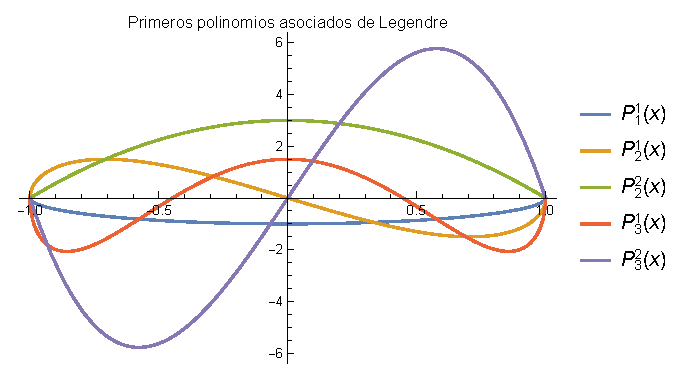
\includegraphics[scale=1.2]{Imagenes/Plot_Asociados_Lagrange.eps}
    \caption{Gráfica de los primeros polinomios asociados de Legendre, no se incluyen aquellos con $m = 0$.}
    \label{fig:figura_asociados_Legedre}
\end{figure}
Debemos de mencionar que las funciones asociadas de Legendre de segunda clase $Q_{\ell}^{m} (x)$ como las $Q_{\ell}(x)$ son singulares en $x = \pm 1$.

\subsection{Propiedades de las funciones asociadas de Legendre \texorpdfstring{$P_{\ell}^{m}$}{Plm}.}

Cuando encontramos en problemas físicos, la variable $x$ de la ecuación asociada de Legendre (como en la ecuación ordinaria Legendre) es generalmente el coseno del ángulo polar $\theta$ en coordenadas polares esféricas, y entonces queremos que la solución $y (x)$ sea regular en $x = \pm 1$ (correspondiente a $\theta = 0$ o $\theta = \pi$). Para que esto ocurra, se requiere que $\ell$ sea un número entero y que el coeficiente $c_{2}$ de la función $Q_{\ell}^{m} (x)$ en la ecuación (\ref{eq:ecuacion_18_31}) sea cero, dado que $Q_{\ell}^{m}(x)$ es singular en $x = \pm 1$, con el resultado de que la solución general son múltiplos de las funciones asociadas de Legendre de primera clase $P_{\ell}^{m}(x)$.

\subsection{Ortogonalidad mutua.}

Ya se mencionó anteriormente que la ecuación asociada de Legendre es del tipo Sturm-Liouville de la forma:
\begin{align*}
\pderivada{(p \, y)} + q \, y + \lambda \,  \omega \, y = 0
\end{align*}
con
\begin{align*}
p &= 1 - x^{2} \\[0.5em]
q &= - \dfrac{m^{2}}{(1 - x^{2})} \\[0.5em]
\lambda &= \ell (\ell + 1) \\[0.5em]
\omega &= 1
\end{align*}
siendo su intervalo natural en $[-1,1]$.
\par
Dado que las funciones asociadas de Legendre $P_{\ell}^{m} (x)$ son regulares en los extremos $x = \pm 1$, entonces deben de ser mutuamente ortogonales en este intervalo para un valor fijo de $m$, es decir:
\begin{align}
\int_{-1}^{1} P_{\ell}^{m} (x) \, P_{k}^{m} (x) \dd{x}  = 0, \hspace{1cm} \mbox{ si } \ell \neq	 k
\label{eq:ecuacion_18_36}
\end{align}
Nótese que el valor de $m$ debe de ser el mismo en ambas funciones asociadas de Legendre para que la expresión sea válida. La condición de normalización cuando $\ell = k$ se obtiene de la fórmula de Rodrigues:
\begin{align}
I_{\ell m} = \int_{-1}^{1} P_{\ell}^{m} (x) \, P_{\ell}^{m} (x) \dd{x} = \dfrac{2}{2 \, \ell + 1} \, \dfrac{(\ell + m)!}{( \ell - m)!}
\label{eq:ecuacion_18_37}
\end{align}
Las condiciones de ortogonalidad y normalización, ecuaciones (\ref{eq:ecuacion_18_36}) y (\ref{eq:ecuacion_18_37}), respectivamente, significan que los polinomios asociados de Legendre $P_{\ell}^{m}(x)$, con $m$ fija, puede utilizarse de manera similar a los polinomios de Legendre para expandir cualquier función $f(x)$ razonable en el intervalo $\abs{x} < 1$ en una serie de la forma:
\begin{align}
f(x) = \nsum_{k=0}^{\infty} a_{m+k} \, P_{m+k}^{m} (x)
\label{eq:ecuacion_18_38}
\end{align}
donde los coeficientes están dados por:
\begin{align*}
a_{\ell} = \dfrac{2 \, \ell + 1}{2} \, \dfrac{(\ell - m)!}{(\ell + m)!} \scaleint{6ex}_{\bs -1}^{1} f(x) \, P_{\ell}^{m} (x) \dd{x}
\end{align*}

\subsection{Función generatriz.}

La función generatriz para las funciones asociadas de Legendre, se obtienen de la combinación de su definición con la función generatriz de los polinomios ordinarios de Legendre:
\begin{align}
G(x, h) = \dfrac{(2 \, m)(1 - x^{2})^{m/2}}{2^{m} \, m! \, (1 - 2 \, h \, x + h^{2})^{m+1/2}} = \nsum_{n=0}^{\infty} P_{n+m}^{m} (x) \, h^{n}
\label{eq:ecuacion_18_40}
\end{align}

\subsection{Relaciones de recurrencia.}

Como era de esperar, las funciones asociadas de Legendre satisfacen ciertas relaciones de recurrencia. De hecho, la presencia de los dos índices $n$ y $m$ significa que se puede derivar una gama mucho más amplia de relaciones de recurrencia. Presentaremos sólo cuatro de las relaciones más útiles:
\begin{align*}
P_{n}^{m+1} &= \dfrac{2 \, m \, x}{(1 - x^{2})^{1/2}} P_{n}^{m} + [m (m - 1) - n (n + 1)] \, P_{n}^{m-1} \\[0.5em]
(2 \, n + 1) \, x \, P_{n}^{m} &= (n + m) \, P_{n-1}^{m} + (n - m + 1) \, P_{n+1}^{m} \\[0.5em]
(2 \, n + 1)(1 -  x^{2})^{1/2} P_{n}^{m} &= P_{n+1}^{m+1} - P_{n-1}^{m+1} \\[0.5em]
2 \, (1 - x^{2})^{1/2} \pderivada{(P_{n}^{m})} &= P_{n}^{m+1} - (n + m)(n - m + 1) \, P_{n}^{m-1}
\end{align*}
Las relaciones de recurrencia son válidas tanto para valores negativos como positivos de $m$. Estas relaciones pueden recuperarse de distintas formas, las cuales incluyen la función generatriz (\ref{eq:ecuacion_18_40}) o diferenciando las relaciones de recurrencia de los polinomios ordinarios de Legendre $P_{\ell}(x)$.

\section{Ejercicios a cuenta.}

\noindent
\textbf{Ejercicio a cuenta (42)} Demuestra que:
\begin{align*}
P_{2n}^{1} (0) &= 0 \\[0.5em]
P_{2n+1}^{1} (0) &= (-1)^{n} \, \dfrac{(2 \, n +1)!}{(2^{n} \, n!)^{2}} = (-1)^{n} \, \dfrac{(2 \, n + 1)!!}{(2 \, n)!!}
\end{align*}
ocupando \textbf{ocupando cada uno} de los siguientes tres métodos:
\begin{enumerate}[label=(\alph*)]
\item Usando relaciones de recurrencia.
\item Expandiendo la función generatriz.
\item Mediante la fórmula de Rodrigues.
\end{enumerate}

\noindent
\textbf{Ejercicio a cuenta (43)} Demuestra que evaluando el $P_{n}^{m}(0)$, se obtiene:
\begin{align*}
P_{n}^{m} (0) = \begin{cases}
(-1)^{\frac{(n-m)}{2}} \, \dfrac{(n + m)!}{2^{n} \bigg[ \left( \dfrac{n - m}{2} \right)! \left( \dfrac{n + m}{2} \right)! \bigg]}, & n + m \mbox{ par} \\
0, & n + m \mbox{ impar}
\end{cases}
\end{align*}
Demuestra adicionalmente que con $n + m$ par, el valor de $P_{n}^{m}(0)$ también se expresa como:
\begin{align*}
P_{n}^{m}(0) = (-1)^{\frac{(n-m)}{2}} \, \dfrac{(n + m - 1)!!}{(n - m)!!}
\end{align*}

\end{document}